\documentclass[11pt]{article}
\usepackage[margin=1in]{geometry}
\usepackage{amsmath}
\usepackage{graphicx}
\usepackage{booktabs}
\usepackage{hyperref}
\graphicspath{{../Figures/}{../Analysis/}}

\title{Result 2.0 Preliminary 2D Spectroscopy Report}
\author{}
\date{}

\begin{document}
\maketitle

\section{Purpose of the test}
This preliminary test applies the Result 2.0 workflow to the supplied minimal bright-dark SOC notebook. The goal is to verify that the model can be wrapped in a stable result-generation interface, produce linked data and figures, and create analysis-ready artifacts without performing an \texttt{Eta} scan. The generated run is a single minimal bright-dark scenario with fixed \texttt{Eta = 0.001} and \texttt{V0 = 0.01 eV}.

\section{Physical model}
The source notebook defines a three-level orbital sector, $|g\rangle$, $|D\rangle$, $|B\rangle$, optionally coupled to an effective spin-Peierls mode. For this test the active scenario keeps the model in the minimal bright-dark limit: \texttt{N\_k = 1}, \texttt{n\_bosons = 1}, \texttt{delta\_0 = 0}, \texttt{Lambda\_SOC = 0}, and zero dissipation. The bright-dark static mixing is set by \texttt{V0 = 0.01 eV}. The solver backend is dense, and the frequency grid is $300 \times 300$.

\section{Trend definitions}
No trend scan is performed in this test. The only scan axis is \texttt{scenario}, with index 0 corresponding to \texttt{minimal\_bright\_dark}. The \texttt{Eta} parameter is fixed in the solver parameters and is not scanned. The quadrant convention is explicit: rephasing is evaluated with $\omega_1 < 0$ and $\omega_3 > 0$, while unrephasing is evaluated with $\omega_1 > 0$ and $\omega_3 > 0$.

\section{Scenarios and acceptance criteria}
\begin{table}[h]
\centering
\begin{tabular}{llll}
\toprule
Scenario & Scan name & Index & Purpose \\
\midrule
minimal\_bright\_dark & scenario & 0 & Single-run workflow and spectrum-production check \\
\bottomrule
\end{tabular}
\caption{Scenario used for the preliminary Result 2.0 workflow test.}
\end{table}

The acceptance criteria for this preliminary test are: the spectra file is saved, all stored arrays are finite, the six mandatory 2D figures exist, rephasing and unrephasing are evaluated in their correct frequency quadrants, and physical trend validation remains inconclusive until at least one control or scan is generated.

\section{Numerical results}
The generated run identifier is \verb|step02__scenario-000__minimal_bright_dark__V0-0p01eV|. The raw spectra and parameter record are saved in the \verb|Data/| folder using this run identifier. The rephasing maximum absolute response is 1.960963e+06, and the unrephasing maximum absolute response is 1.970183e+06.

\begin{figure}[h]
\centering
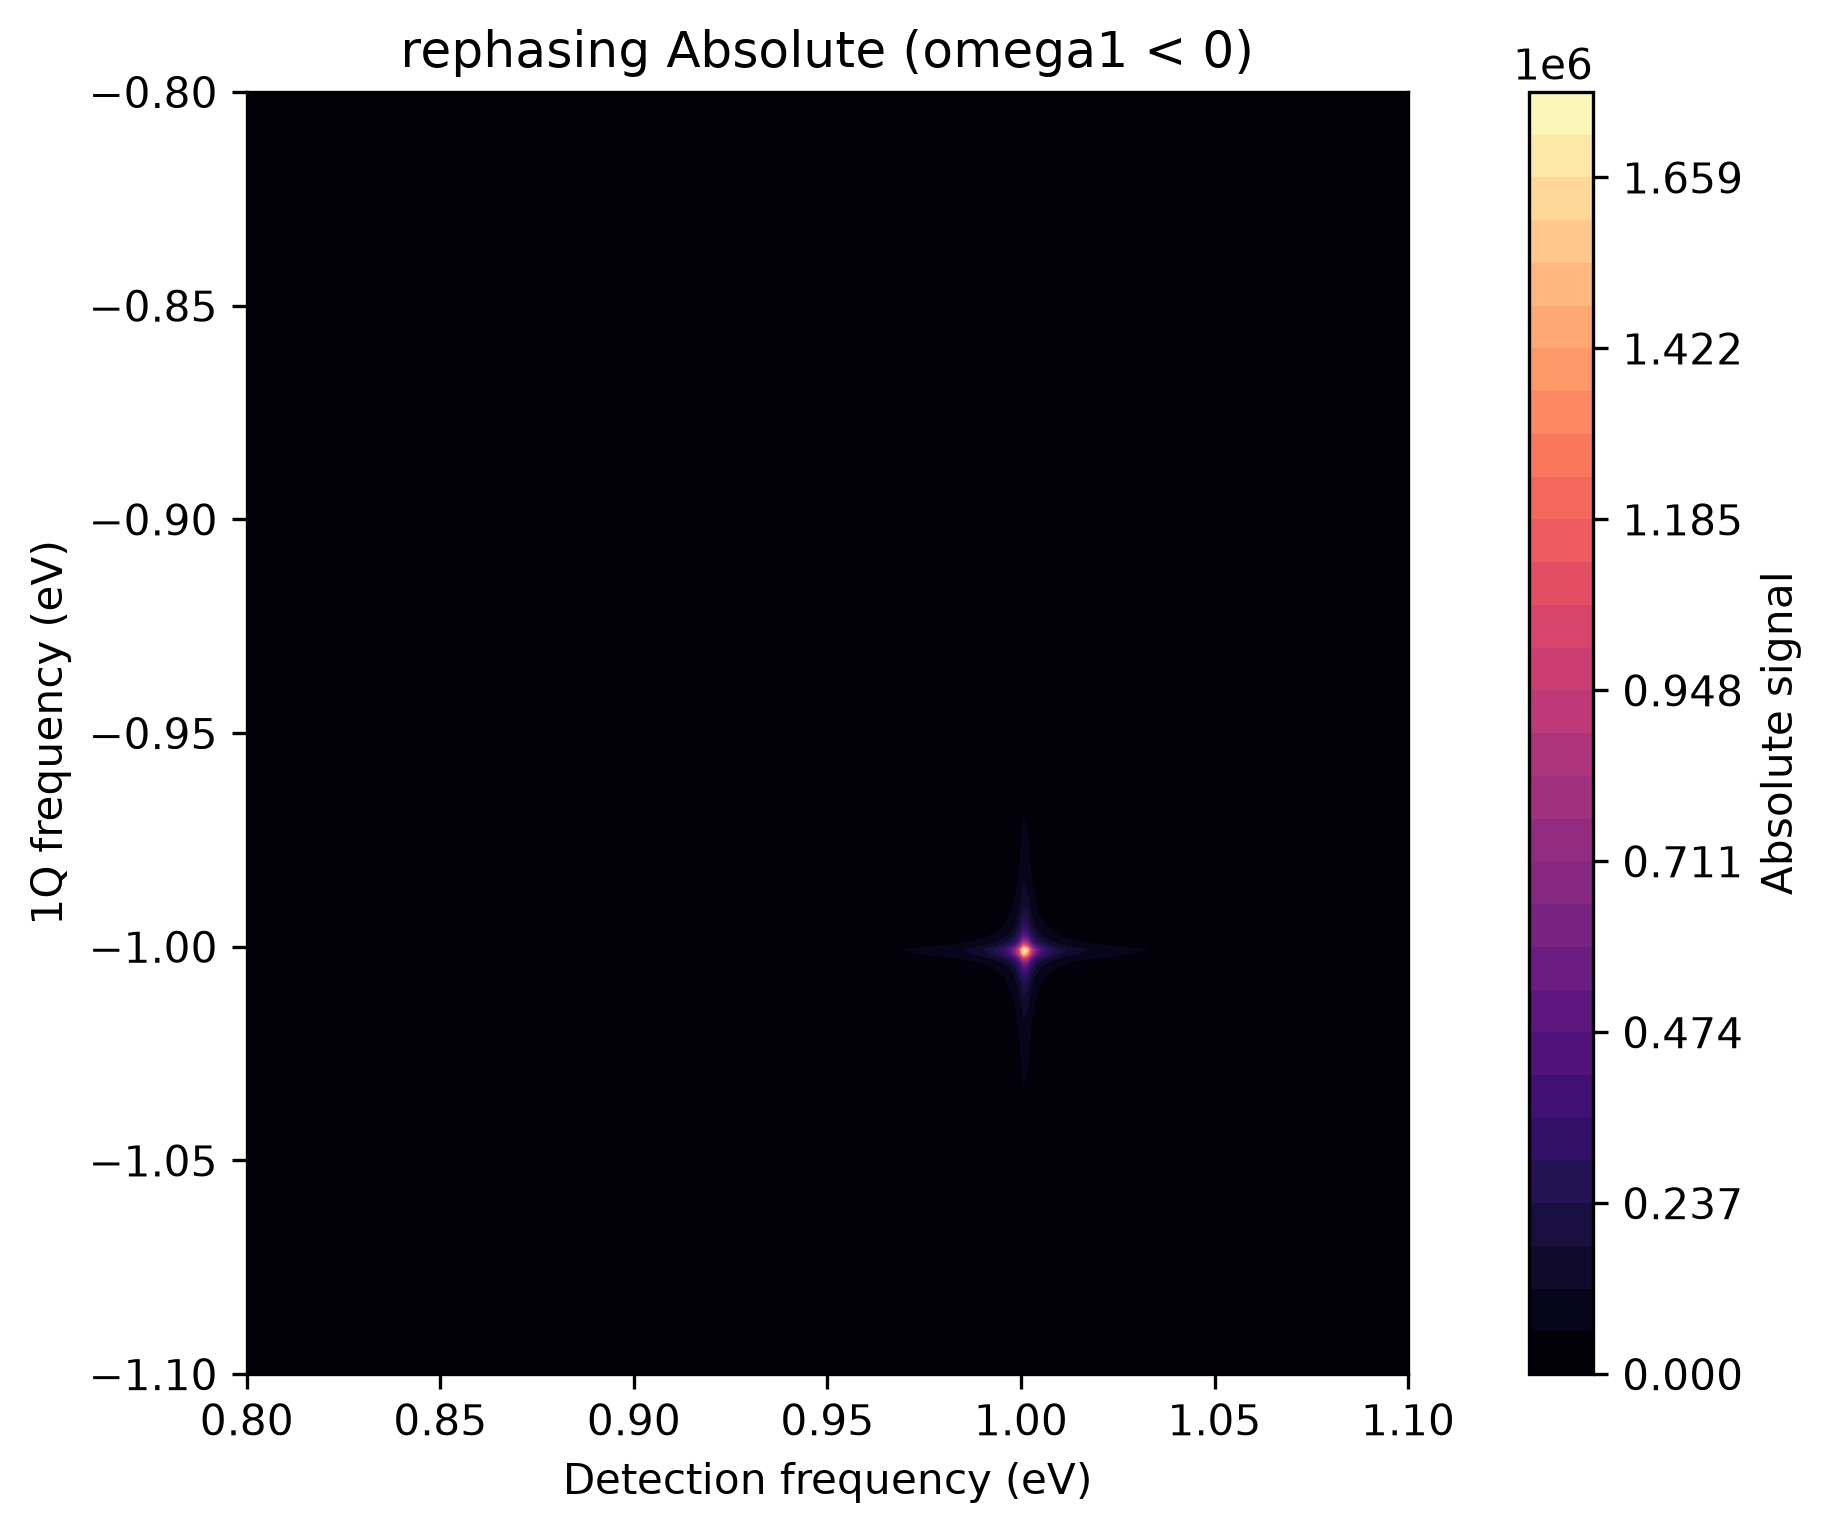
\includegraphics[width=0.48\textwidth]{step02__scenario-000__minimal_bright_dark__V0-0p01eV_rephasing_abs.png}
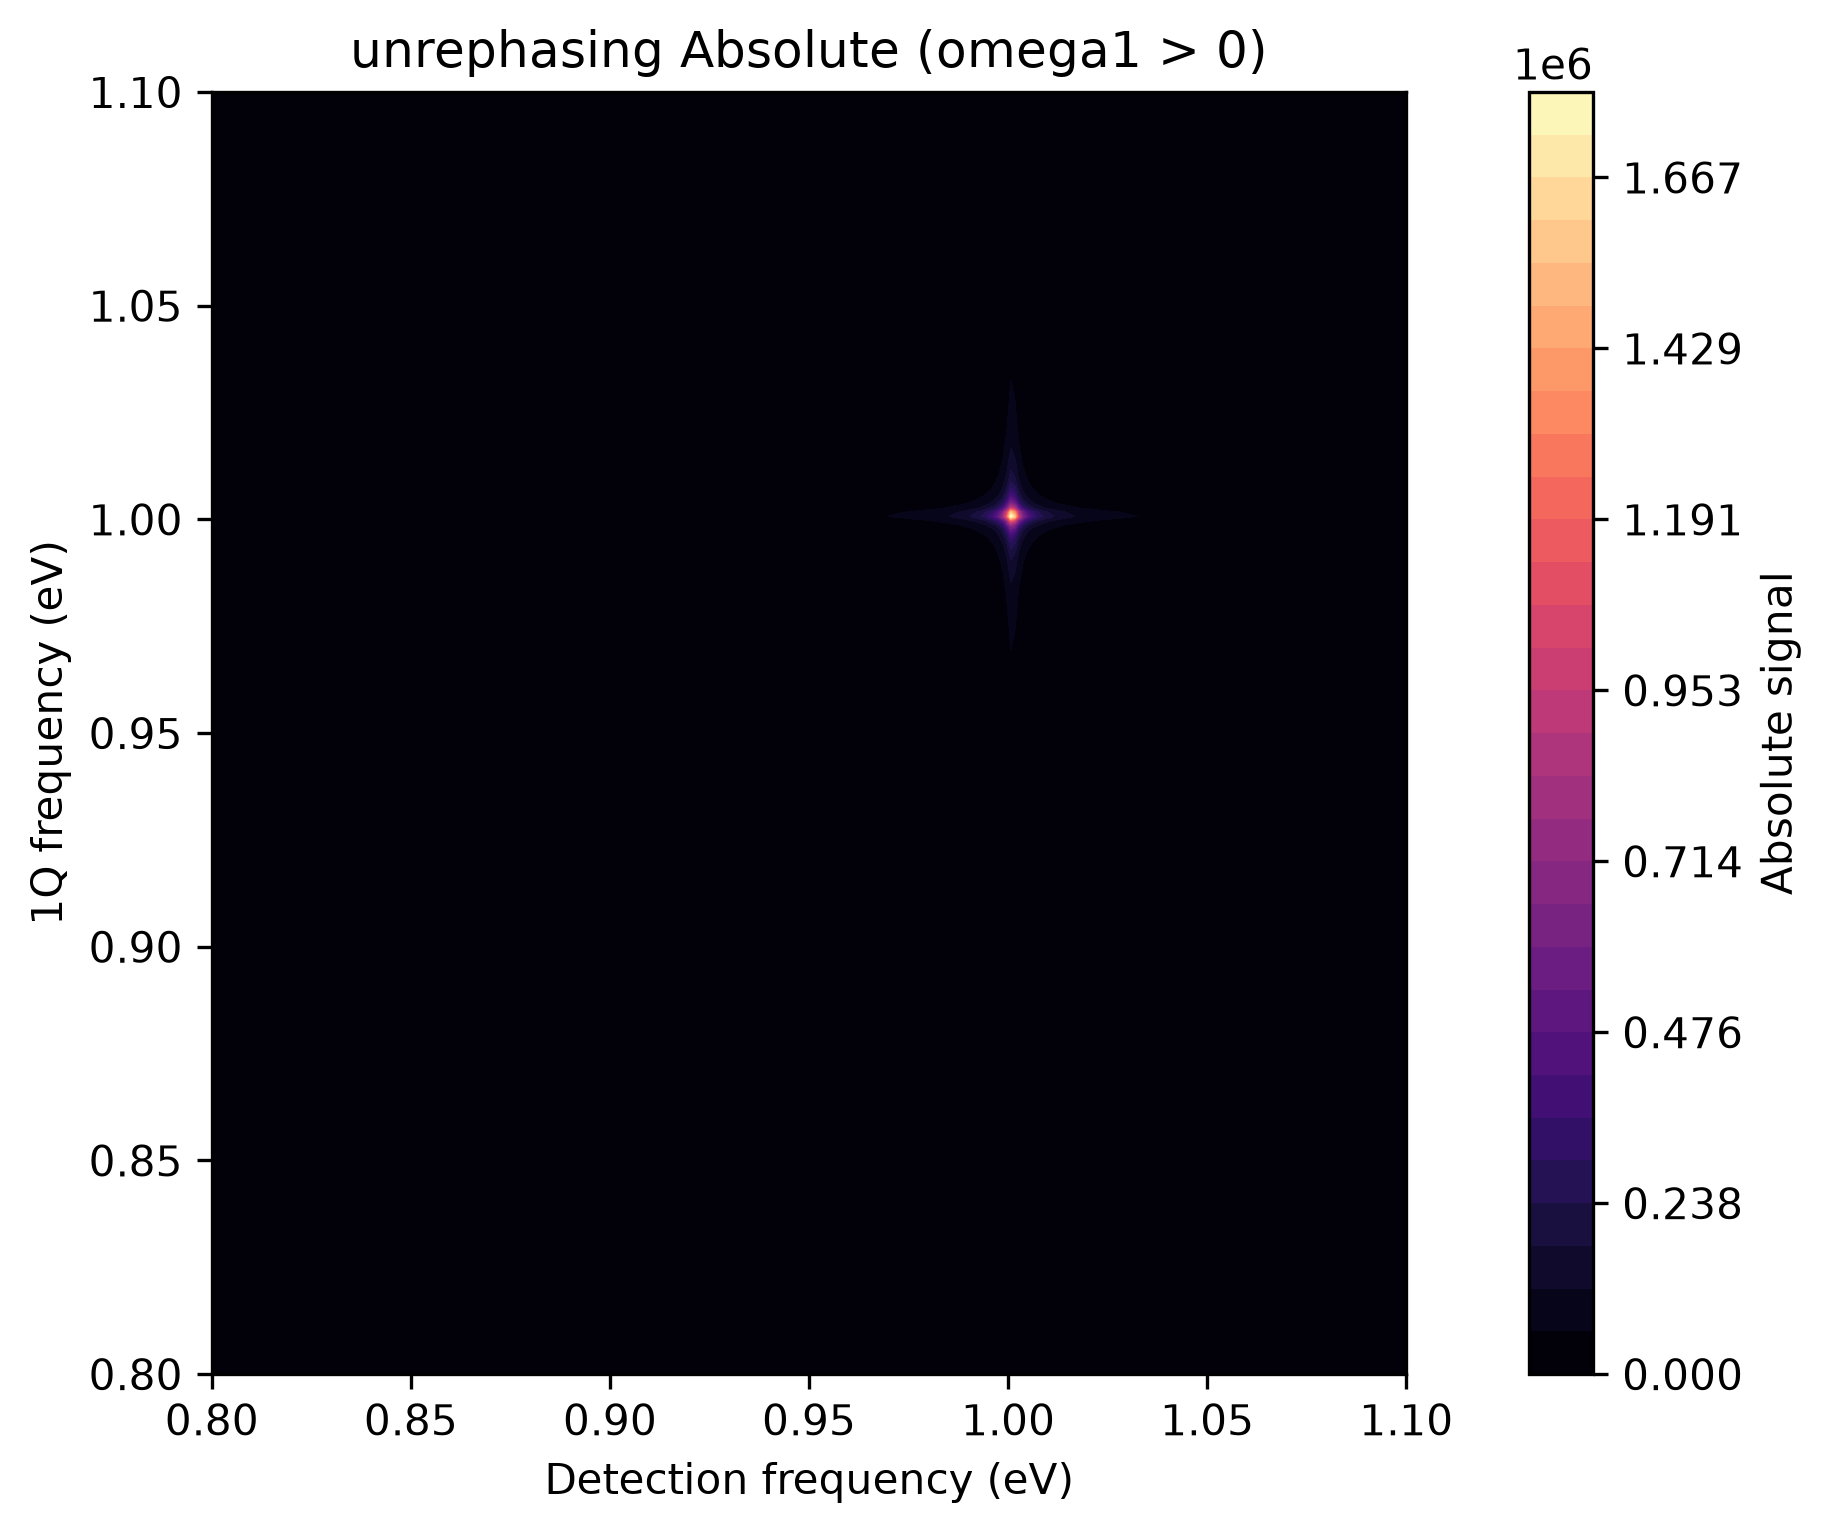
\includegraphics[width=0.48\textwidth]{step02__scenario-000__minimal_bright_dark__V0-0p01eV_unrephasing_abs.png}
\caption{Absolute 2D spectra for the minimal bright-dark scenario. Left: rephasing quadrant $\omega_1 < 0$. Right: unrephasing quadrant $\omega_1 > 0$.}
\end{figure}

\begin{figure}[h]
\centering
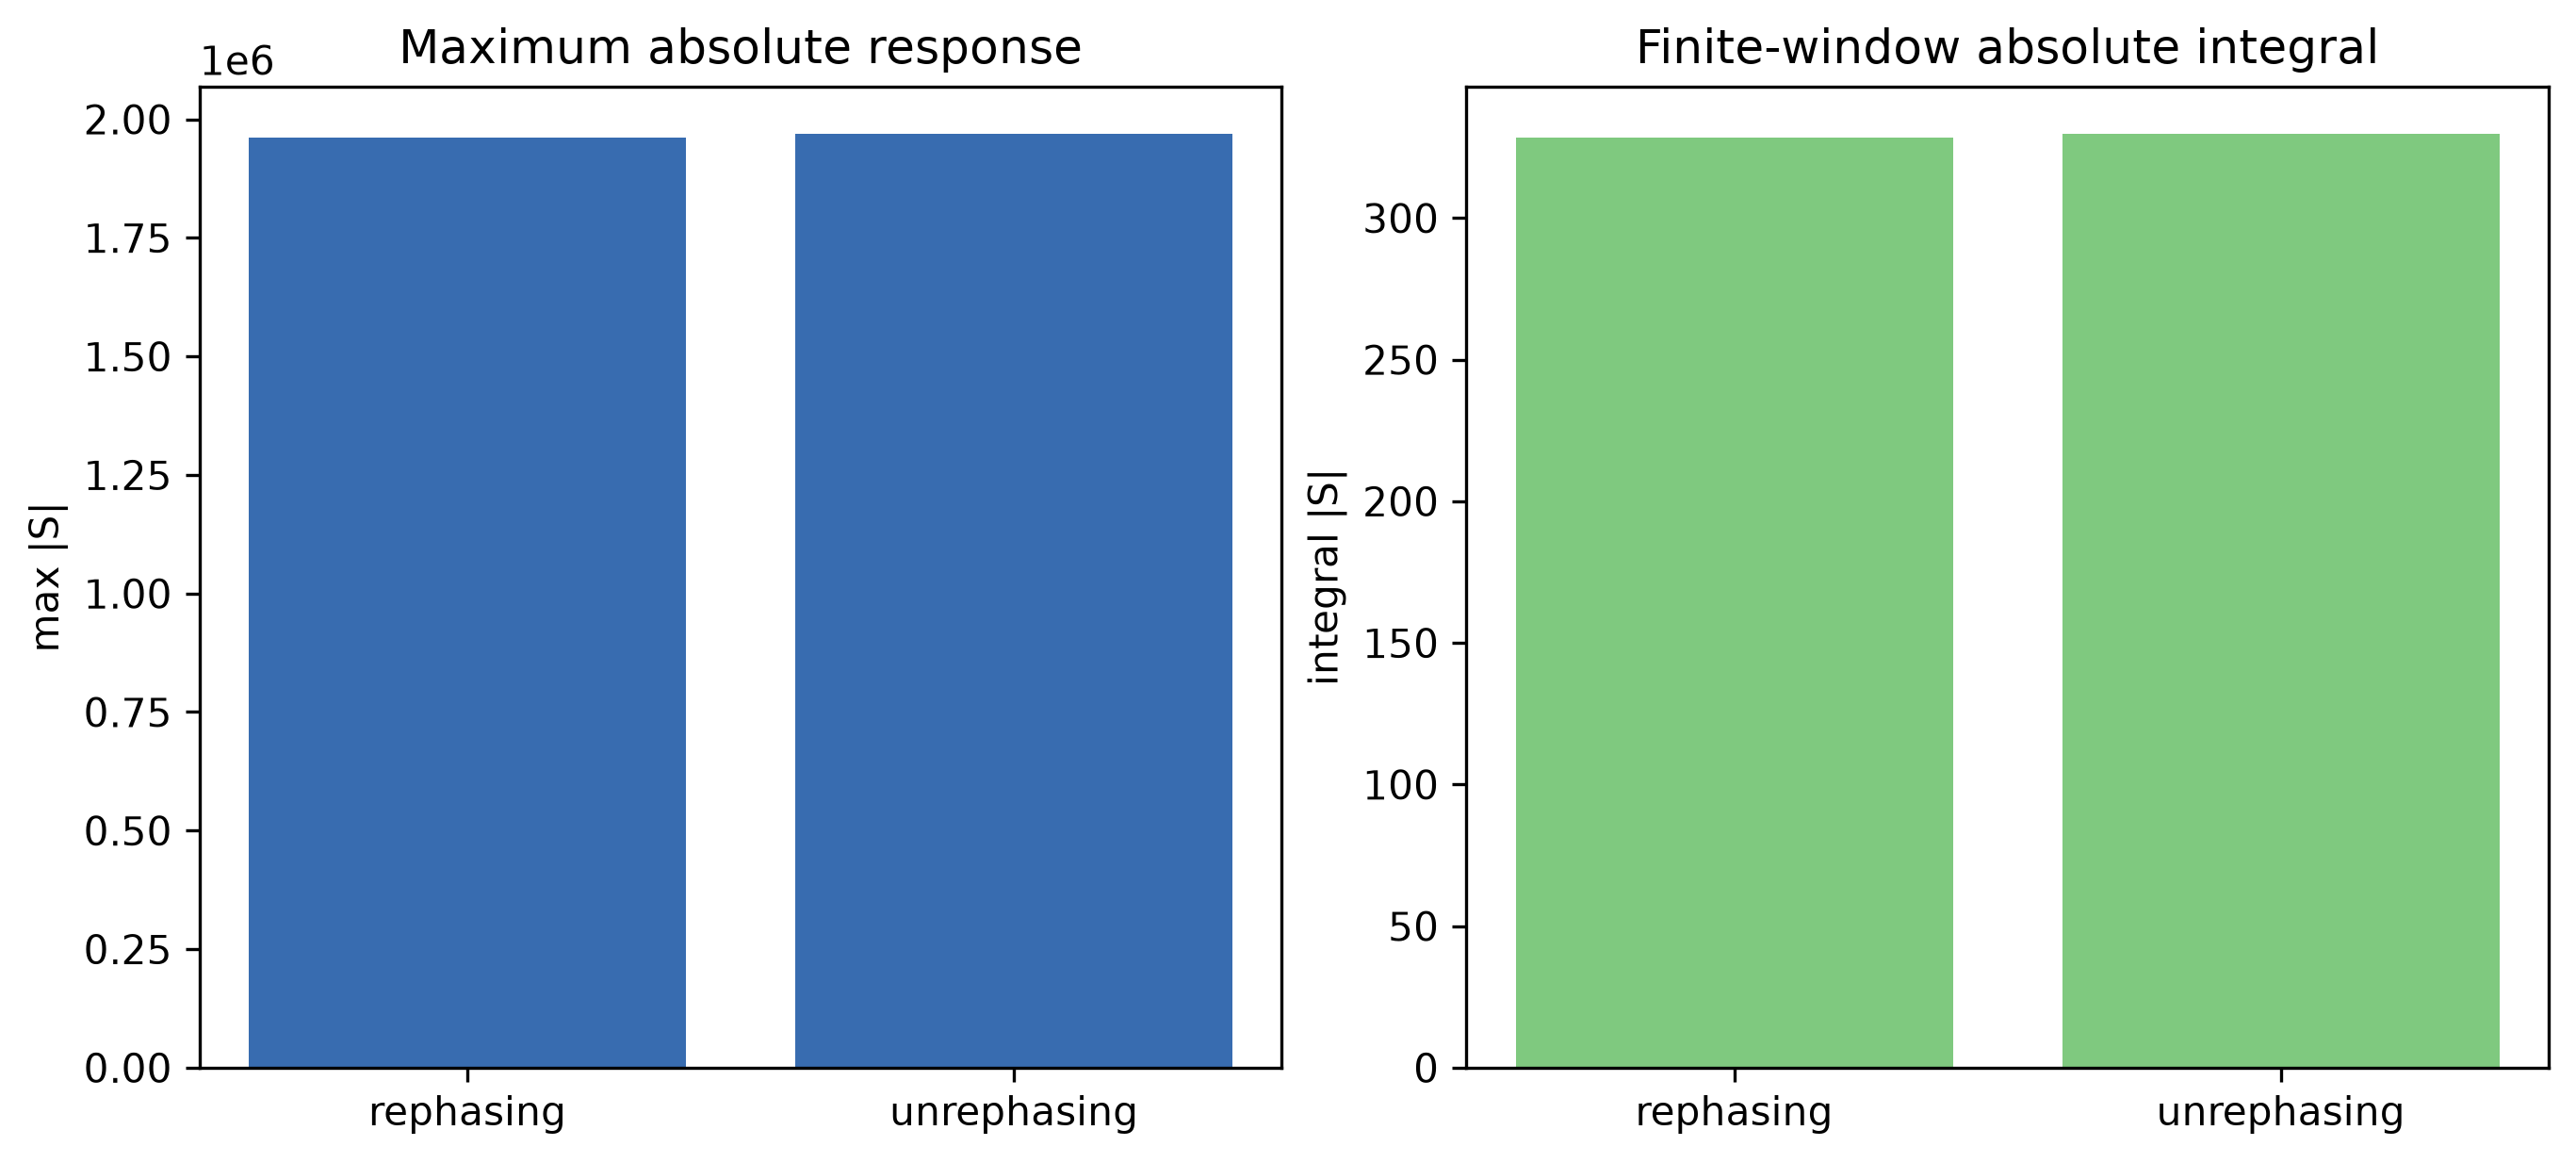
\includegraphics[width=0.80\textwidth]{step02__scenario-000__minimal_bright_dark_metric_summary.png}
\caption{Analysis summary for the generated rephasing and unrephasing components.}
\end{figure}

\section{Validation outcome}
The result-production criteria pass: the spectra file exists, the stored arrays are finite, all six mandatory figures were produced, and the rephasing/unrephasing frequency quadrants are correct. The physical trend criterion is \texttt{INCONCLUSIVE} because only one scenario was generated. A trend-level validation would require at least one control scenario or a scan over a physically meaningful parameter such as field, temperature, or bright-dark mixing.

\end{document}
